\ifnum \Version=1
    \question[7] Consider the non-linear system below.  
    \begin{align*}
        \dxdt &= y(x+y-4) , \qquad \dydt = x(2x+y-6)
    \end{align*}
    \begin{parts}
        \part Determine the locations of the critical points. 
        \ifnum \Solutions=1 {\color{DarkBlue} \\[12pt] 
        Setting both $x'=0$ and $y'=0$, we obtain four critical points as follows. $x'=0$ implies $y=0$ or $x+y-4=0$. 
            \begin{itemize}
                \item If $y=0$, then for $y'=0$ we need either $x=0$ or $2x+y-6=0$. 
                \begin{itemize}
                    \item If $y=0$ and $x=0$, one critical point is at $(0,0)$. 
                    \item If $y=0$ and $2x+y-6=0$, one critical point is at $(3,0)$. 
                \end{itemize}
                \item If $x+y-4=0$, then for $y'=0$ we need either $x=0$ or $2x+y-6=0$. 
                \begin{itemize}
                    \item If $x+y-4=0$ and $x=0$, one critical point is at $(0,4)$. 
                    \item If $x+y-4=0$ and $2x+y-6=0$, then solving this system of equations yields a critical point at $(2,2)$. 
                \end{itemize}                
            \end{itemize}
            The four critical points are located at $(0,0)$, $(3,0)$, $(0,4)$, $(2,2)$. 
            } 
        \else 
        \vfill
        \fi
        \part Sketch the nullclines of the system on the axes below. Clearly indicate the critical points that you found in part (a). 
        \ifnum \Solutions=1 {\color{DarkBlue} \\[12pt] 
        Green lines are the $x-$nullclines, blue lines are the $y-$nullclines.
        \begin{center}
        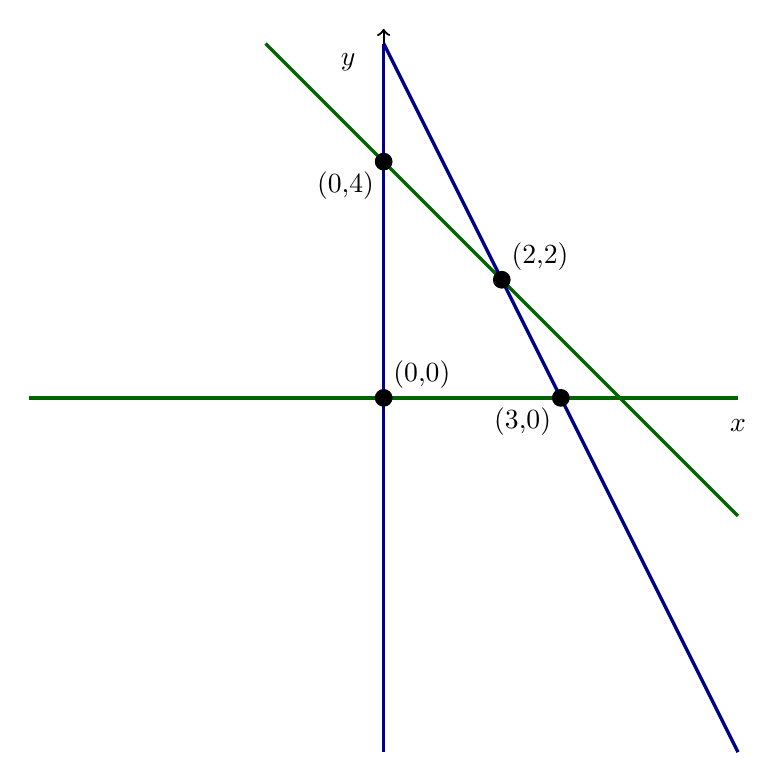
\begin{tikzpicture}[scale=0.75]
        % \draw[thick, ->] (-6, 0) -- (6.25, 0);
        \draw[thick, ->] (0, -6) -- (0, 6.25);
        \node[overlay, below] at (6, -0.2) {$x$};
        \node[overlay, below] at (-0.6, 6) {$y$};   
        \draw[very thick,DarkGreen, -] (-2, 6) -- (6, -2);        
        \draw[very thick,DarkGreen, -] (-6, 0) -- (6, 0);   
        \draw[very thick,DarkBlue, -] (0, 6) -- (6, -6);        
        \draw[very thick,DarkBlue, -] (0, -6) -- (0, 6);      
        \filldraw[black] (0,0) circle (4pt) node[anchor=south west]{(0,0)};
        \filldraw[black] (0,4) circle (4pt) node[anchor=north east]{(0,4)};
        \filldraw[black] (2,2) circle (4pt) node[anchor=south west]{(2,2)};
        \filldraw[black] (3,0) circle (4pt) node[anchor=north east]{(3,0)};
        \end{tikzpicture}
        \end{center}            
        } 
        \else 
        \begin{center}
        \begin{tikzpicture}[scale=0.55]
        \draw[very thick, ->] (-6, 0) -- (6.25, 0);
        \draw[very thick, ->] (0, -6) -- (0, 6.25);
        \node[overlay, below] at (6, -0.2) {$x$};
        \node[overlay, below] at (-0.6, 6) {$y$};        
        \end{tikzpicture}
        \end{center}    
    \fi
    \end{parts}
\fi 

